\section{Applications de la détection des valeurs aberrantes sur des problèmes réel}
 \textcolor{red}{En construction}
%Perhaps an image (see Figure~\ref{fig:Cities}?
%\begin{figure*}[t]
 %   \centering
 %   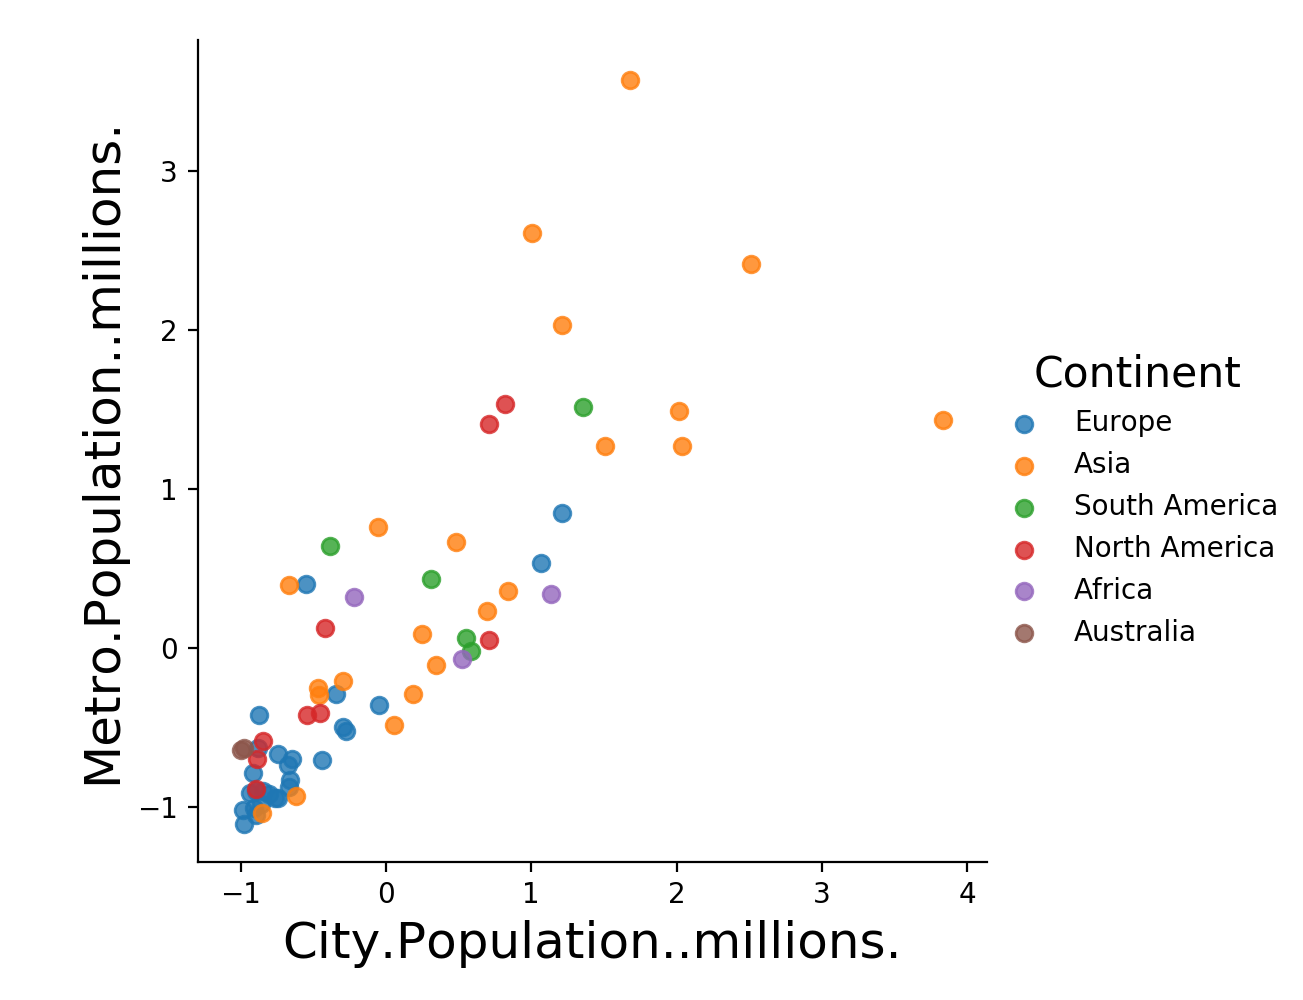
\includegraphics[width=.40\textwidth]{ADOA/Images/CityPopu.png}
 %   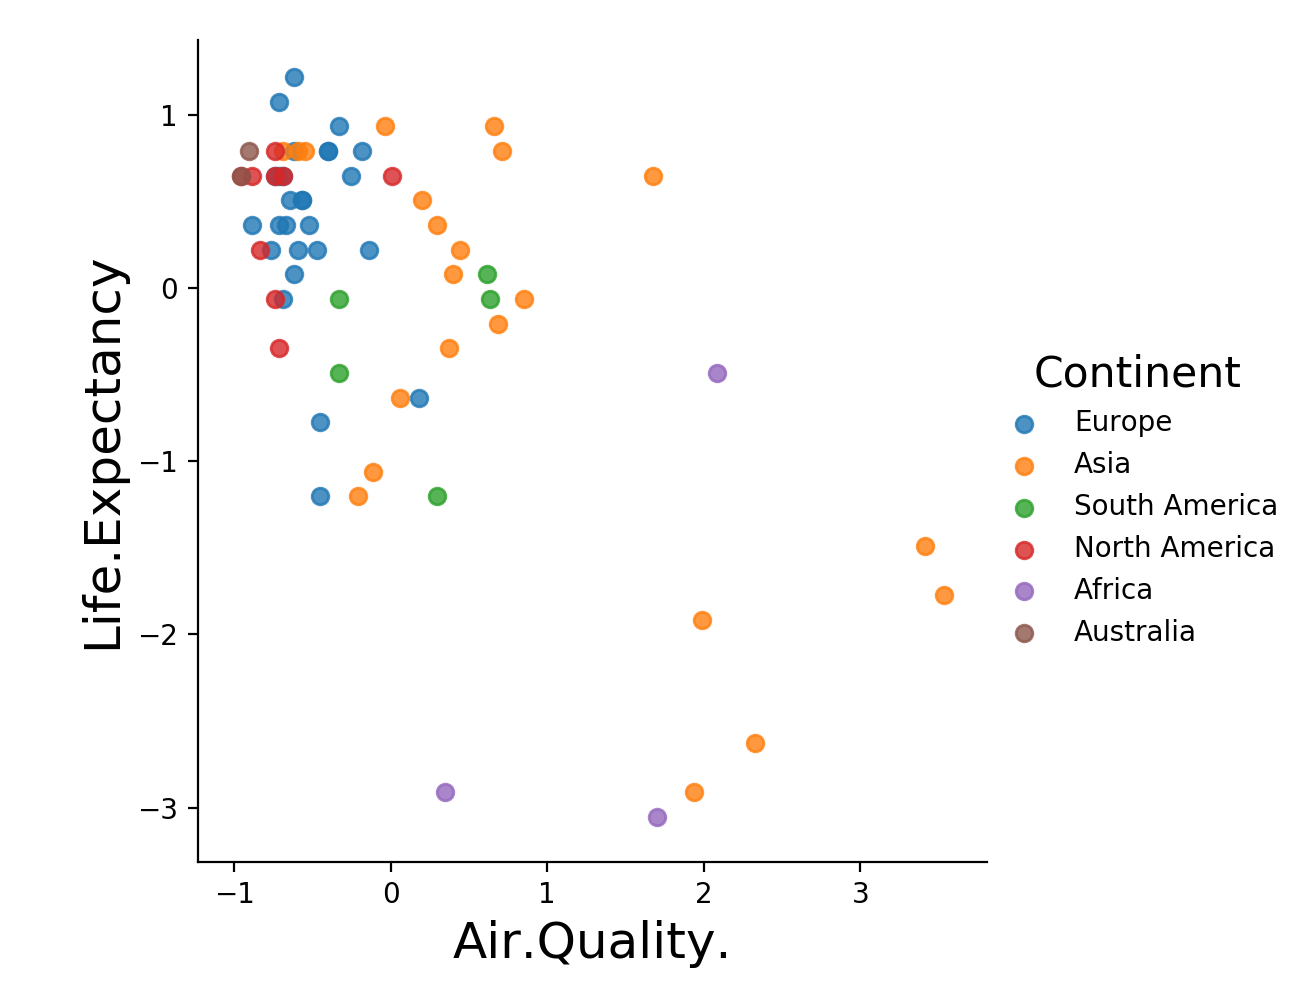
\includegraphics[width=.4\textwidth]{ADOA/Images/AirquaLifeExp.png}
 %   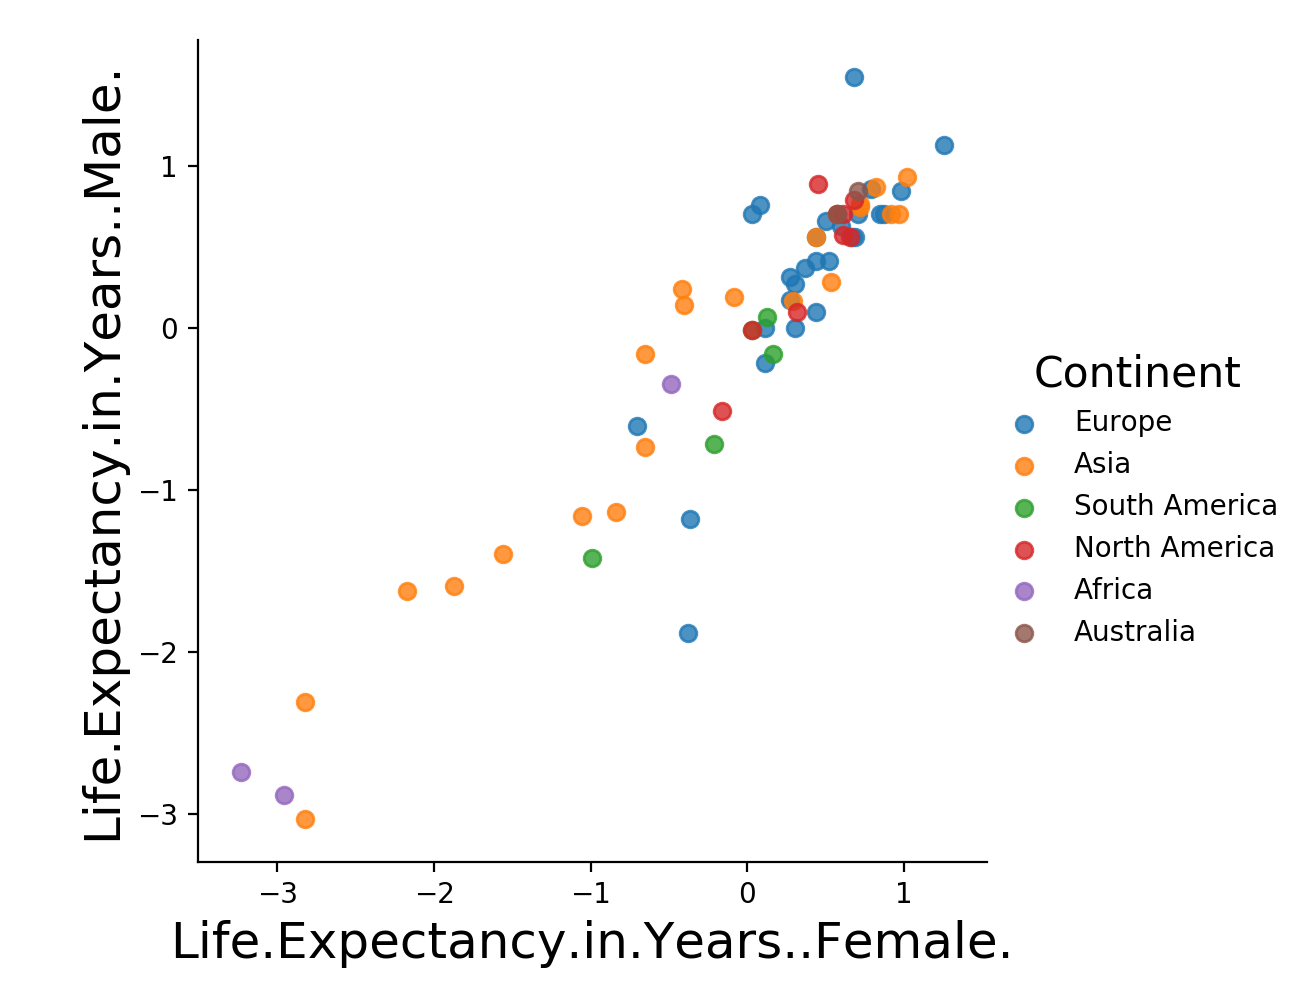
\includegraphics[width=.4\textwidth]{ADOA/Images/LifeExpMaleFemale.png} %
 %   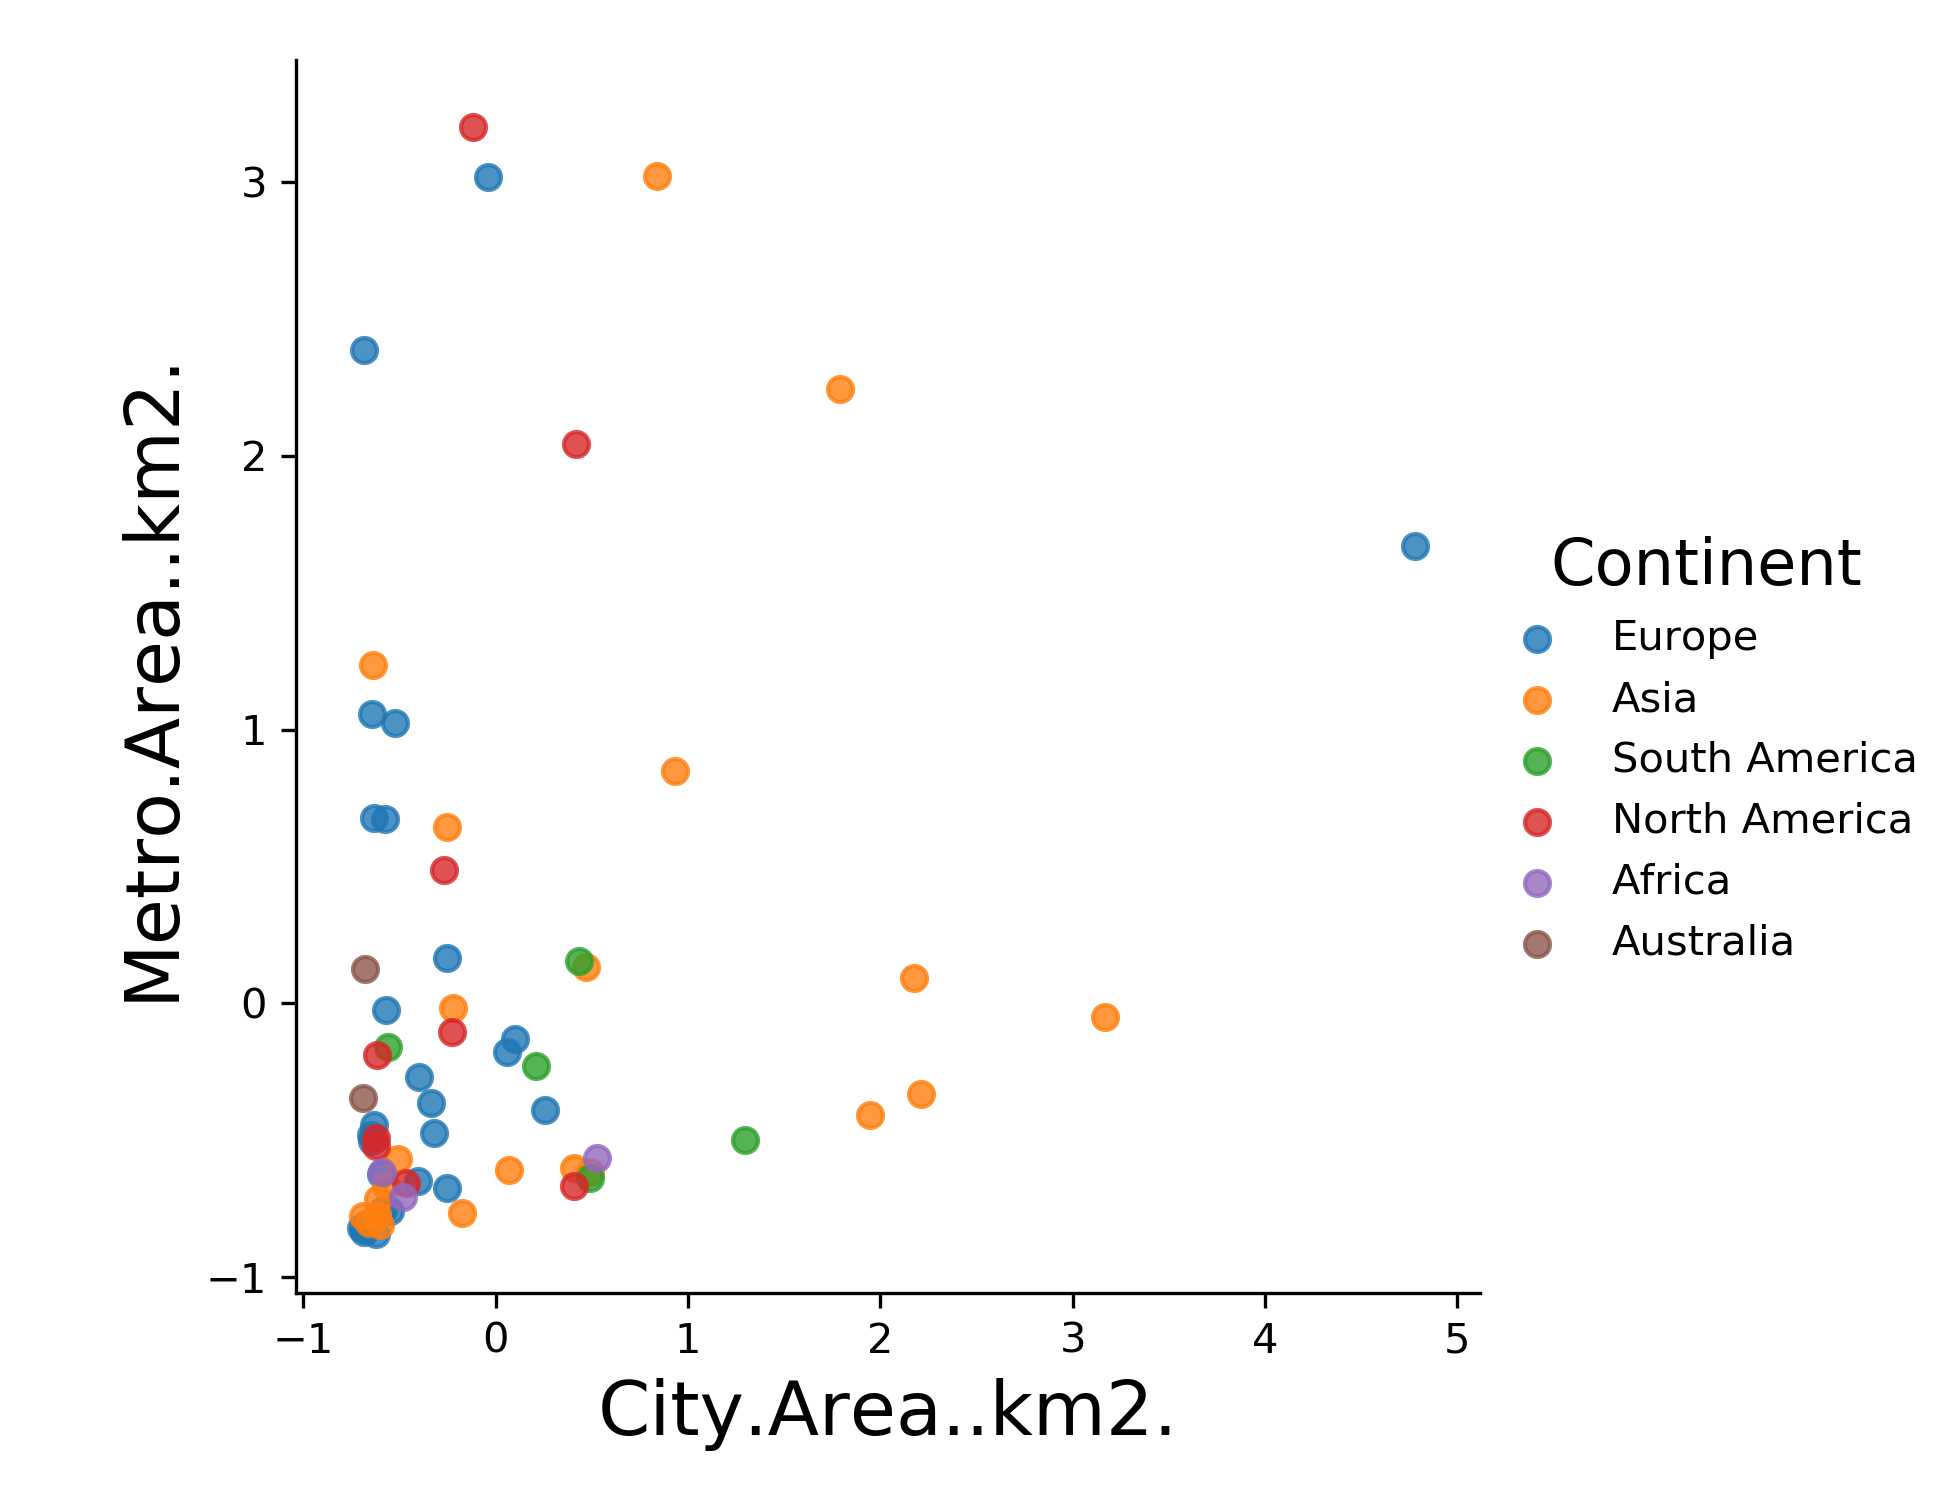
\includegraphics[width=.4\textwidth]{ADOA/Images/CityAreaMetro.png} 
 %   \caption{.}\hrule
 %   \label{fig:Cities}
%\end{figure*}
%\begin{figure*}[t]
%    \centering
%    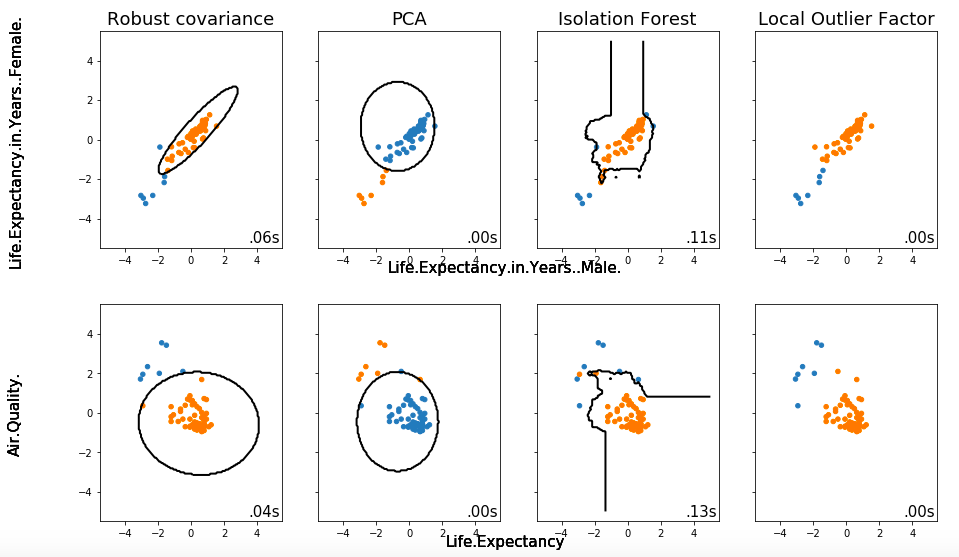
\includegraphics[width=\textwidth]{ADOA/Images/Allcomp1.png}
%    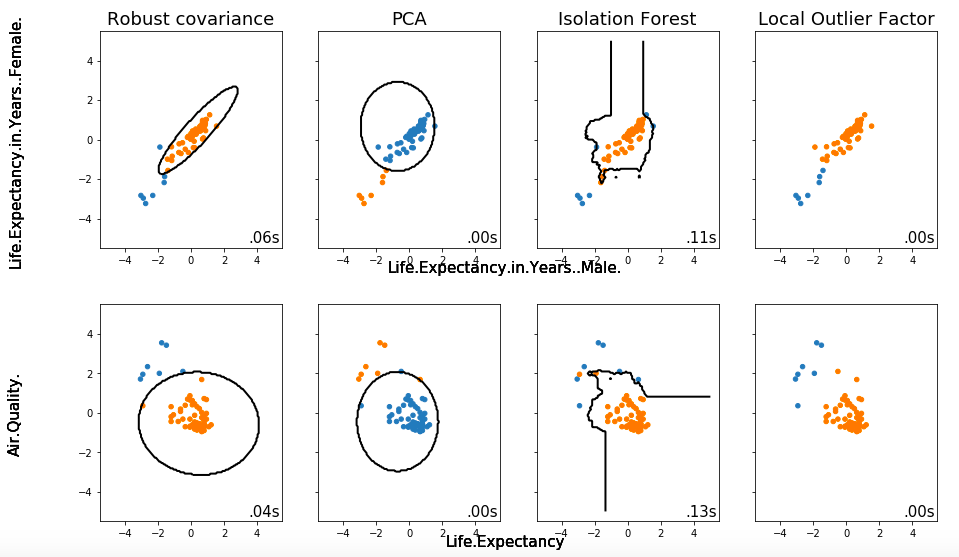
\includegraphics[width=\textwidth]{ADOA/Images/Allcomp1.png}
%
%    \caption{.}\hrule
%    \label{fig:Cities}
%\end{figure*}
\subsection{Contrôle de qualité}
\subsection{Finance}